%!TEX root = ../../Principal/TFG.tex
\chapter{ Anexo II: Visualizaci�n de los vectores de caracter�sticas con la herramienta PCA}
\label{appe:C}
\pagestyle{fancy}
\thispagestyle{empty}
%
\graphicspath{{../ApendiceC/Imagenes/}}
\DeclareGraphicsExtensions{.pdf,.png,.jpg}
%


Si visualizamos los vectores de caracter�sticas obtenidos durante la fase de reclutamiento utilizando la herramienta PCA (an�lisis de componentes principales, ACP, en castellano), las agrupaciones por usuario, que ve�amos bien definidas en el espacio con la herramienta TSNE, dejan de ser tan evidentes, y solo un reducido n�mero de usuarios parece estar distanciado del resto. 
\newline

\begin{figure}[h!]
	\centering
	\subfigure[MODELO 1]{
		\label{fig:pca1}
		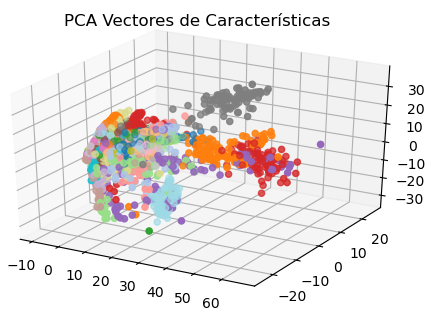
\includegraphics[width=0.32\textwidth]{/pca1}}
	\subfigure[MODELO 2]{
		\label{fig:pca2}
		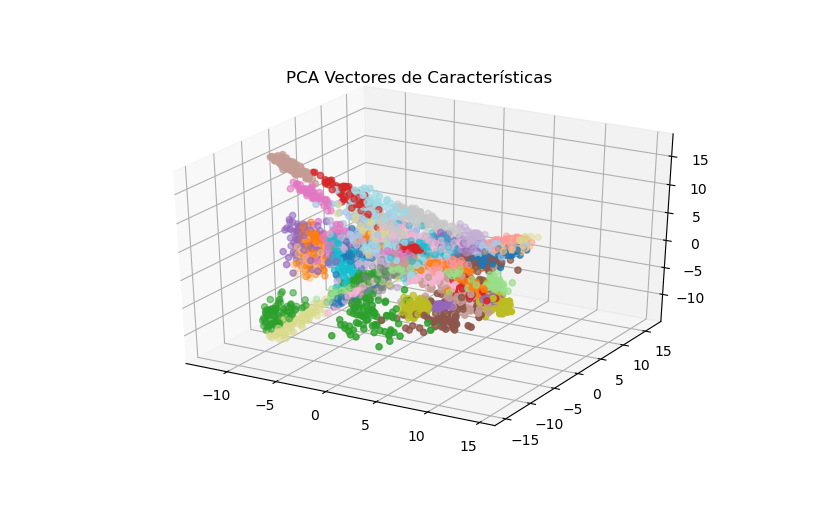
\includegraphics[width=0.32\textwidth]{/pca2}}
	\subfigure[MODELO 3]{
		\label{fig:pca3}
		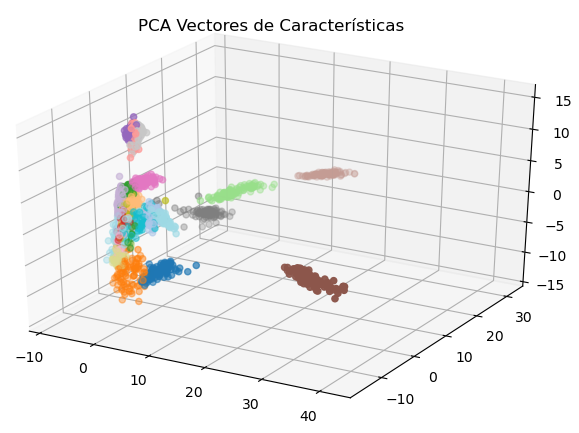
\includegraphics[width=0.32\textwidth]{/pca3}}
	\caption{Comparativa de la distribuci�n de los vectores de caracter�sticas obtenidos durante la fase de reclutamiento para cada modelo, empleando la herramienta de visualizaci�n PCA para reducir a tres dimensiones el espacio.}
	\label{pca}
\end{figure}